\subsection{UC1 - Gestione autenticazione}
\begin{itemize}
    \item \textbf{Identificativo}: UC1
    \item \textbf{Nome}: Gestione autenticazione
    \item \textbf{Descrizione grafica}:
\end{itemize}

\begin{center}
    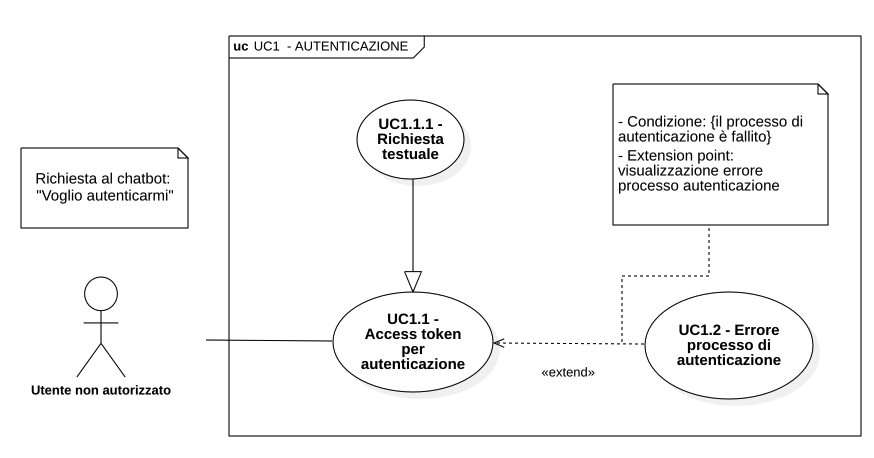
\includegraphics[scale=0.50]{images/UC1.png} 
\end{center}

 \begin{itemize}
    \item \textbf{Attori}
 \begin{itemize} 
    \item \textit{Primari}: utente non autorizzato
    \item \textit{Secondari}: non presenti
 \end{itemize}
 \item \textbf{Precondizione}: l'utente non dispone di un token\textsubscript{G} di accesso per poter effettuare l'autenticazione con il chatbot.
 \item \textbf{Postcondizione}:il chatbot risponde alla richiesta dell'utente fornendo un link attraverso il quale l'utente può ottenere il token\textsubscript{G} di accesso ai servizi messi a disposizione dal chatbot.
 \item \textbf{Scenario principale}: l'utente deve effettuare il login al sistema, fa una richiesta scritta (\textbf{UC1.1.1}) oppure vocale (\textbf{UC1.1.2}) alle quali il bot risponde fornendo un link per effettuare l'autenticazione (\textbf{UC1.1}). Se l'utente prova ad autentificarsi con un token\textsubscript{G} di accesso non valido viene visualizzata una schermata di errore. (\textbf{UC1.2})
\end{itemize}
\newpage

\subsubsection{UC1.1 - Token di accesso autenticazione}
\begin{itemize}
    \item \textbf{Identificativo}: UC1.1
    \item \textbf{Nome}: token\textsubscript{G} di accesso autenticazione
    \item \textbf{Descrizione grafica}: (approfondita in UC1)
    \item \textbf{Attori}
 \begin{itemize} 
    \item \textit{Primari}: utente non autorizzato
    \item \textit{Secondari}: non presenti
 \end{itemize}
 \item \textbf{Precondizione}: l'utente ha a disposizione un token\textsubscript{G} di accesso.
 \item \textbf{Postcondizione}: l'utente fornisce il token\textsubscript{G} al chatbot.
 \item \textbf{Scenario principale}: se il token\textsubscript{G} fornito è valido allora l'utente avrà effettuato il login correttamente e potrà usufruire dei sistemi messi a disposizione. Se il token\textsubscript{G} non risulta valido, verrà mostrato un messaggio di errore ad esso relativo (\textbf{UC1.2})
\end{itemize}

\subsubsection{UC1.2 - Token non valido}
\begin{itemize}
    \item \textbf{Identificativo}: UC1.2
    \item \textbf{Nome}: token\textsubscript{G} non valido
    \item \textbf{Descrizione grafica}: (approfondita in UC1)
    \item \textbf{Attori}
 \begin{itemize} 
    \item \textit{Primari}: utente non autorizzato 
    \item \textit{Secondari}: non presenti
 \end{itemize}
 \item \textbf{Precondizione}: l'utente ha a disposizione un token\textsubscript{G} non valido.
 \item \textbf{Postcondizione}: chatbot nega l'accesso ai servizi, viene comunicato l'errore all'utente e riproposto il sistema di login.
 \item \textbf{Scenario principale}: il token\textsubscript{G} inserito dall'utente risulta essere non valido per l'accesso, viene mostrato un messaggio di errore e il chatbot propone all'utente di rieffettuare la procedura di login.
\end{itemize}
\newpage